\documentclass[a4paper,10pt]{article}
\usepackage[utf8x]{inputenc}
\usepackage[lithuanian]{babel}
\usepackage[L7x]{fontenc}
\usepackage{lmodern}
\usepackage{verbatim}
\usepackage{tocloft} 
\usepackage{url}
\renewcommand{\cftsecleader}{\cftdotfill{\cftdotsep}}
\usepackage{parskip}
\usepackage{graphicx} 
\parindent = 1cm
\usepackage{mathtools} % pades rašyti matematinius intarpus


\begin{document}
\maketitle
%\begin{titlepage}

\begin{center}
VILNIAUS UNIVERSITETAS\\
MATEMATIKOS IR INORMATIKOS FAKULTETAS\\
PROGRAMŲ SISTEMŲ KATEDRA\\
\vspace{150pt}

\huge \textbf{Daugiamačių duomenų klasifikavimo analizė\\}
\vspace{20pt}
\large\textbf{Classification analysis of high-dimensional data\\}
\vspace{20pt}
\small Bakalauro darbas\\
\vspace{40pt}
\end{center} 


\begin{flushleft}
Atliko: \hspace{50pt} Dainius Jocas \hspace{105pt}\textsubscript{(para\v{s}as)}

\vspace{10pt}
Darbo vadovas: \hspace{12pt} Dr. Juozas Gordevičius \hspace{65pt}\textsubscript{(para\v{s}as)}

\vspace{10pt}
Darbo recenzentas: Dr. Vardenis Pavardenis \hspace{50pt}\textsubscript{(para\v{s}as)}
\\
\vspace{130pt}
\end{flushleft}

\begin{center}
VILNIUS - 2012
\end{center}

\end{titlepage}


%\begin{titlepage}

\begin{center}
VILNIAUS UNIVERSITETAS\\
MATEMATIKOS IR INORMATIKOS FAKULTETAS\\
PROGRAMŲ SISTEMŲ KATEDRA\\
\vspace{150pt}

\huge \textbf{Daugiamačių duomenų klasifikavimo analizė\\}
\vspace{20pt}
\large\textbf{Classification analysis of high-dimensional data\\}
\vspace{20pt}
\small Bakalauro darbas\\
\vspace{40pt}
\end{center} 


\begin{flushleft}
Atliko: \hspace{50pt} Dainius Jocas \hspace{105pt}\textsubscript{(para\v{s}as)}

\vspace{10pt}
Darbo vadovas: \hspace{12pt} Dr. Juozas Gordevičius \hspace{65pt}\textsubscript{(para\v{s}as)}

\vspace{10pt}
Darbo recenzentas: Dr. Vardenis Pavardenis \hspace{50pt}\textsubscript{(para\v{s}as)}
\\
\vspace{130pt}
\end{flushleft}

\begin{center}
VILNIUS - 2012
\end{center}

\end{titlepage} % kol kas neaktualu
\let \savenumberline \numberline
\def \numberline#1{\savenumberline{#1.}}
%\tableofcontents 
\begin{comment}
%% JG: Sekcija apie darbe nagrinėjamą problemą. Problem definition.

\section{Teorija}
Šiame skyriuje aptarsiu teorinį darbo pagrindą ir pagrindus.
\subsection{Mokymasis su mokytoju ir mokymasis be mokytojo}

Mašininis mokymasis yra dirbtinio intelekto šaka, kuri siekia įgalinti kompiuterius tobulinti savo elgseną (mokytis) empirinių duomenų atžvilgiu \cite{duda2001pattern}. Pagal tai, kokie yra turimi empiriniai duomenys, mašininis mokymasis yra skirstomas į mokymąsi su mokytoju (angl. \textit{supervised learning}) ir mokymąsi be mokytojo (angl. \textit{unsupervised learning}). Šiame poskyryje aptarsiu, kas yra mokymasis su mokytoju ir mokymasis be mokytojo bei kuo jie skiriasi.

\subsubsection{Mokymasis su mokytoju}

Žmonės mokosi iš patirties, tačiau, skirtingai nei žmonės, kompiuteris patirties neturi, todėl kompiuteris turi mokytis iš patyrimą apibūdinančių duomenų -- mokymosi duomenų. Mašininio mokymosi tikslas yra sukonstruoti funkciją, kuri galėtų būti naudojama nuspėti patyrimą apibūdinančių charakteristikų reikšmes pagal patyrimą apibūdinančius duomenis. Mokymesi su mokytoju, mokytoją reikia suprasti kaip išankstinį mokymosi duomenų spėjamų charakteristikų žinojimą. Kitaip tariant, mokymesi su mokytoju yra sprendžiamas uždavinys, kuriam atsakymą galime pasitikrinti. Pagal tai, kokias charakteristikas bandome nuspėti mokymasis su mokytoju yra skirstomas į dvi rūšis:
\begin{enumerate}
  \item Klasifikavimas (angl. classification) -- pagal mokymosi duomenų nepriklausomus kintamuosius bandoma nuspėti kokybinius (kategorinėd reikšmės) priklausomus kintamuosius.
  \item Regresinė analizė (angl. regression) -- pagal mokymosi duomenų nepriklausomus kintamuosius bandoma nuspėti kiekybinius (tolydinėd reikšmės) priklausomus kintamuosius.
\end{enumerate} 

%% JG: Pateik vizualų klasifikavimo pavyzdį iliustruojanti visus 3 etapus.
%% DJ: Vizualų, ta prasme su paveiksliukais ar ir tas pavyzdys su paštu pakankamai vaizdingas?
%% JG: Reikia kitaip struktūrizuoti šitą skyrių: 
% +Pradžioj pasakyk, kad yra klasifikavimas ir regresija ir po
%  sakinįÂ kiekvienam.
% +Tada aptark klasifikavimą ir pateik pavyzdį. 
% +Tada pateik regresijos pavyzdį.
% +Tada parašyk, kad šiame darbe studijuojama klasifikavimo problema.

\paragraph{Klasifikavimas}

Mašininiame mokymesi klasifikavimu yra vadinama problema, kai pagal mokymosi duomenis reikia nustatyti, kuriai klasei (grupei) priklauso objektas. Klasifikavimo procesas pavaizduotas ~\ref{fig:classification_process} pav. pavaizduota srautų diagrama. Dirbant su biomedicininiais duomenimis tipinė užduotis yra pagal mėginį (pacientą) apibūdinančius matus (patirtį) sukonstruoti klasifikatorių (funkciją), kuris bandys nuspėti, kuriai pacientų grupei -- sergančiųjų ar sveikųjų -- priklauso tiriamasis pacientas.
\begin{figure}
 \centering
 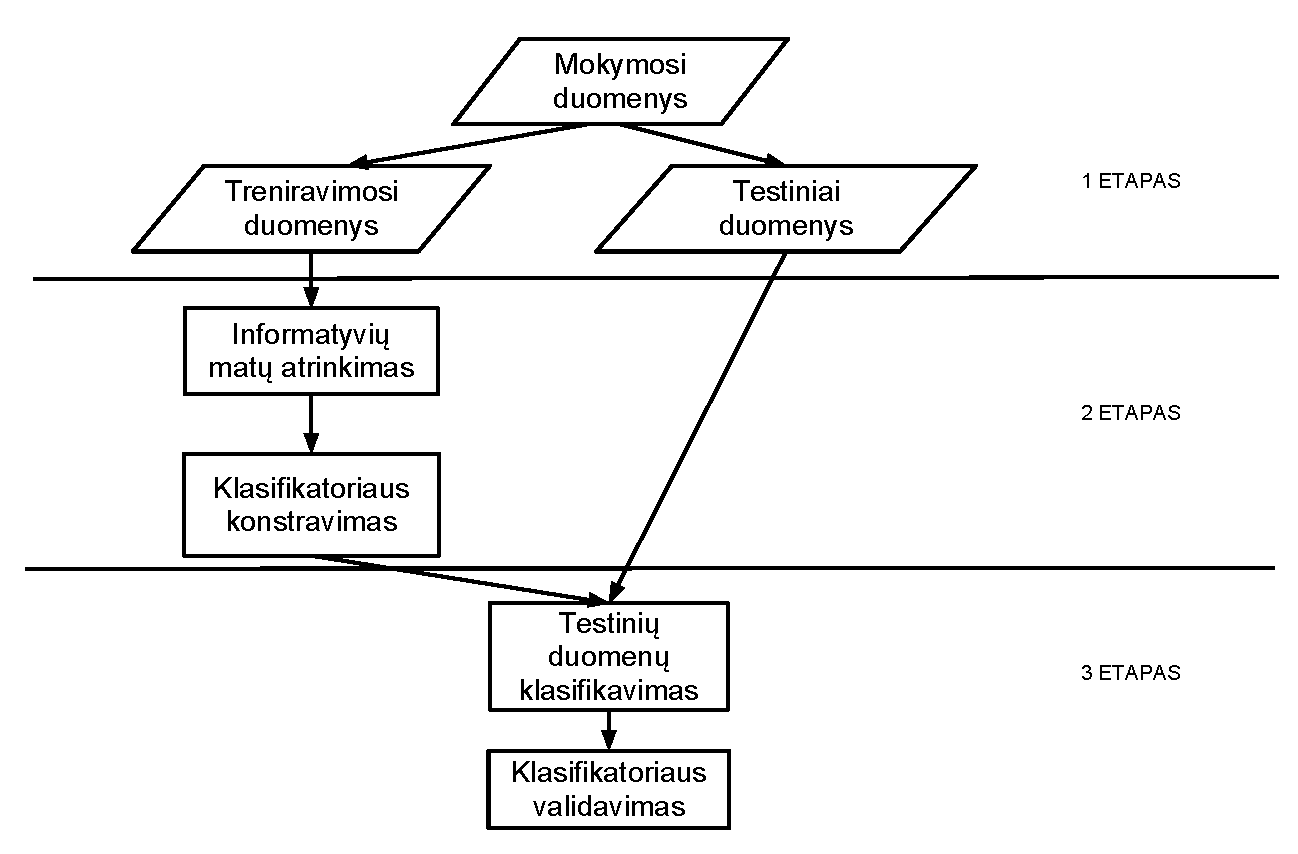
\includegraphics[width=\textwidth]{images/classification_process.pdf}
 \caption{Klasifikavimo srautų diagrama su paaiškinimais.}
 \label{fig:classification_process}
\end{figure}

\paragraph{Regresinė analizė}

Mašininiame mokymesi regresine analize yra vadinama problema, kai pagal patirtį apibūdinančius duomenis reikia nustatyti kiekybines duomenų charakteristikas. Regresinė analizė naudoja standartinius statistinius metodus, tokius kaip mažiausių kvadratų metodas (angl. \textit{least squares}). Regresinė analizė dažniausiai naudojama įvertinti (ang. \textit{forecast}) ateities duomenų vertes bei interpoliacijai -- funkcijos tikėtinos reikšmės tarp keletos taškų įvertinimui. 

Dirbant su biomedicininiais duomenimis regresinė analizė gali būti taikoma bandant nuspėti mėginių trūkstamus matus apibūdinančias reikšmes -- interpoliuoti. Tačiau regresinė analizė dirbant su biomedicininiais duomenimis yra naudojama rečiau negu klasifikavimas, todėl toliau šiame darbe bus nagrinėjama klasifikavimo problema.

%% DJ: Juozai, gal turi gražų pavyzdį, kur pritaikoma regresinė analizė dirbant su biomedicininiais duomenimis?

\subsubsection{Mokymasis be mokytojo}

Mašininio mokymosi kontekste dažnai sutinkamas uždavinys yra į prasmingas grupes (klasterius) sugrupuoti turimus duomenis, apie kuriuos nieko nėra žinoma. Kitaip tariant, reikia išspręsti duomenų grupavimo uždavinį, kuriam neturima iš anksto teisingo atsakymo. Mokymasis be mokytojo tai toks mokymasis, kai teisingas mokymosi duomenų grupavimas iš anksto nėra žinomas. Mokymosi be mokytojo pagrindinis principas -- maksimizuoti objektų, esančių toje pačioje grupėje, tarpusavio panašumą ir minimizuoti tarpgrupinį objektų panašumą.

Mokymosi su mokytoju metu galima išmatuoti gautos funkcijos tikslumą įvairiais metodais, pvz. kryžminiu patikrinimu (angl. \textit{cross-validation}). Mokymosi be mokytojo proceso rezultato tiesioginio patikrinimo procedūrų nėra. Todėl yra sunku išsiaiškinti rezultatų, gautų pagal mokymosi be mokytojo algoritmų darbo rezultatus, patikimumą. 

% Yra mažiausiai penkios pagrindinės priežastys, kodėl mums gali būti įdomūs mokymosi be mokytojo algoritmai:
% \begin{enumerate}
%   \item Turime labai daug nesužymėtų (angl. \textit{unlabelled}) duomenų, o jų sužymėjimas rankomis būtų labai brangus. 
%   \item Norime apsimokyti su dideliu kiekiu sąlyginai ,,pigių`` duomenų tam, kad paskui galėtume pasitelkti mokymosi su mokytoju algoritmus, ir tada detaliau ištirti duomenis.
%   \item Duomenų struktūros šablonas yra nuolat kintantis, ir jei tą kitimą galėtume sekti mokymosi be mokytojo režimu, tai būtų galima padidinti mūsų programos našumą.
%   \item Galima panaudoti mokymosi be mokytojo algoritmus, kad surastume duomenų savybes, kurias vėliau panaudosime duomenų kategorizavimui.
%   \item Pradinėje duomenų analizės stadijoje pasinaudoję mokymosi be mokytojo metodais galime geriau pažinti turimus duomenis.
% \end{enumerate}

%% JG: neprižiūrimų mokymosi metodų yra visokių: association rule mining,
% clustering, ir t.t. Zr ESL knygos 14 skyrių.
%% DJ: Nurašinėjau nuo Duda knygos tą vietą, kur mokymas be mokytojo ir 
% klasterizavimas yra sinonimai.

%% Kartais šiokia tokia informacija žinoma. Pvz., klasteriųÂ kiekis nurodomas
% k-means algoritme. Arba galima daryti prielaidas apie klasterių struktūrą:
% k-means ieško apvalių klasterių. Esminis dalykas yra tas, kad teisingas
% atsakymas nėra žinomas.

%% JG: algoritmas turi atrasti grupes duomenyse, jos nėra iš anksto žinomos.

\paragraph{Klasterizavimas}

Klasterizavimas yra viena iš mokymosi be mokytojo algoritmų rūšių. Klasterizavimas -- tai turimų objektų suskirstymas į skirtingas grupes (klasterius) taip, kad grupės viduje esantys objektai būtų panašūs tarpusavyje, o objektai iš skirtingų grupių būtų nepanašūs. Klasterizavimu siekiama atrasti nežinomas struktūras turimuose duomenyse. 

Klasterizavimo algoritmuose mes matuojame objektų panašumą. Panašumui matuoti yra naudojami atstumo tarp objektų metrikos, tokios kaip \textit{Manhattan}, Euklido, \textit{Mahalanobis} atstumai. Tačiau pasirinktosios atstumo metrikos rezultatai priklauso nuo to, kokioje skalėje yra atlikti paskirų matų matavimai. Todėl yra rekomenduojama prieš klasterizavimą visus matus normalizuoti. Dažniausiai naudojamas normalizavimas yra, kai mato matavimų reikšmių vidurkis yra $0$, o standartinio nuokrypio -- $1$ matavimo vienetas (angl. \textit{unit}). Normalizavimu siekiame apsisaugoti nuo situacijos, kai matas su didelėmis reikšmėmis gali iškreipti atstumo matavimus. 

Dirbant su biomedicininiais duomenimis klasterizavimo algoritmus galime panaudoti panašių matų sugrupavimui. Iš panašių matų grupės pasirinkus tik vieną reprezentatyviausią matą, būtų galima sumažinti bendrą matų skaičių. Toks matų skaičiaus sumažinimas pagerintų matų atrinkimo procesą.

\paragraph{Hierarchinis klasterizavimas}

% Šio skyrelio reikia, nes Consensus Group Stable matų atrinkimo metodas naudoja hierarchinio klasterizavimo algoritmą
Hierarchinis klasterizavimas (angl. hierarchical clustering) yra klasterizavimo algoritmas, kuris arba visą duomenų aibę panariui skaido į vis mažesnius klasterius (angl. divisive learning), arba pradeda nuo kiekvieno elemento ir kiekviename etape sujungia panašiausius klasterius (angl. \textit{agglomerative clustering}).  Hierarchinio klasterizavimo rezultatas -- klasterių medis, dendograma, rodanti, kaip klasteriai yra susiję. Pasirinktame lygyje nupjovus dendogramą gaunama pasirinkta klasetrizavimo struktūra \cite{martisiute08}. 

Hierarchinis klasterizavimas yra informatyvesnis nei paprastas -- plokščias -- klasterizavimas.

\subsubsection{Mokymosi su mokytoju ir mokymosi be mokytojo skirtumai}

 Pagrindiniai skirtumai tarp mokymosi su mokytoju ir mokymosi be mokytojo yra:
\begin{itemize}
  \item mokymosi duomenys -- mokymosi su mokytoju proceso įeities duomenyse yra išreikštinai pasakyta, kokio rezultato mes laukiame, o mokymosi be mokytojo įeities duomenyse tokios papildomos informacijos nėra.
  \item  naudojimo tikslai -- mokymasis su mokytoju siekia iš pavyzdžių išmokti vertinti naujus duomenis, o mokymasis be mokytojo siekia atrasti vidinę duomenų struktūrą.
\end{itemize}
Mokymosi su ir be mokytojo procesai panašūs savo esme -- siekia išgauti žinias apie turimus duomenis, tačiau jų panaudojimas skiriasi iš esmės -- mokymosi su mokytoju atveju siekiama išmokti iš pavyzdžių, o mokymosi be mokytojo atveju siekiama atrasti nežinomas struktūras turimuose duomenyse.

%% JG: aš nesutinku, kad abiem procesais siekiama tųÂ pačių tikslų. Vienu atveju 
% siekiama išmokti iš pavyzdžių. Kitu atveju siekiama atrasti nežinomas
% struktūras turimuose duomenyse. Procesai yra panašūs savo esme, bet jų 
% panaudojimas skiriasi iš esmės.

%% JG: iš vikipedijos: In machine learning, unsupervised learning refers to the 
% problem of trying to find hidden structure in unlabeled data. Since the
% examples given to the learner are unlabeled, there is no error or reward
% signal to evaluate a potential solution. This distinguishes unsupervised 
% learning from supervised learning and reinforcement learning.

%% JG: visą šitą skyrių reikia pateikti koncentruotai. Esminiai teiginiai ir grafiniai pavyzdžiai. 

%% DJ: Turiu pripažint, kad šitam pavyzdyje prigrybavau stipriai. Nurašinėjau
% pavyzdį kur prastai paaiškino skirtumą, bet užtat man pavyzdys patiko. Dabar
% labiau į temą surašyta.
 % Supervised and Unsupervised Learning
\subsection{Bajeso teorija}

Kuris terminas geresnis: ,,Bajeso teorija`` ar ,,Bajeso išvadų teorija``?
Arba kaip reikėtų versti ``Bayesian Decision Theory''?
Kaip reikėtų suprasti P(error|x)?
% Sensitivity: measures difficulty of task
% Bias: measures strategy of subject

Bajeso teorija\cite{duda2001pattern} yra statistinis požiūris į modelių (angl.
pattern) klasifikavimo problemą. Bajeso teorija paremta klasifikavimo sprendimų kompromisų (angl.
tradeoff) matavimų tikimybėmis ir tų sprendimų svoriais. Bajeso teorija remiasi
prielaida, kad sprendimą galima aprašyti tikimybiniais teminais ir kad
susijusios tikimybės yra iš anksto žinomos.

Kitaip tariant, Bajeso teorija padeda atsakyti į klausimą, kokią tikimybė, kad
objektas priklauso kažkokiai klasei $\omega_j$ ir jis turi kažkokią savybę $x$.
Tai galime užrašyti taip: 

\begin{equation}
p(\omega_j, x) = P(\omega_j | x) \times p(x) = p(x|\omega_j) \times P(\omega_j)
\end{equation}

O jei pergrupuosime pirmąją formulę, tai gausime taip vadinamąją Bajeso formulę:

\begin{equation}
P(\omega_j | x) = \frac{p(x | \omega_j) \times P(\omega_j)}{p(x)}, kur
\end{equation}

$P(\omega_j | x)$ (angl. posterior probability) - sąlyginė tikimybė,
kad objektas priklauso $\omega_j$ klasei, kai kažkuri jo savybė yra $x$;

$p(x | \omega_j)$ (angl. likelihood) - sąlyginė tikimybė, kad $\omega_j$ klasei
priklausantis objektas turės kažkokią savybę x;

$P(\omega_j)$ (angl. prior probability) - tikimybė, kad objektas priklauso
$\omega_j$ klasei (nusatoma iš istorinių duomenų);

$p(x) = \sum_{j=1}^{n} p(x | \omega_j) \times P(\omega_j)$ (angl. evidence) -
perskaičiavimo faktorius (angl. scale factor), kuris parodo tai, kaip dažnai mes
įvertinsime modelį su savybe $x$. Jis užtikrina, kad visų $P(\omega_j | x)$
sąlyginių tikimybių suma bus lygi 1.

Remdamiesi Bajeso teorija laikysime, kad objektas priklauso klasei $\omega_i$,
kai $P(\omega_i | x) > P(\omega_j | x)$ ir atvikščiai. Tai yra taip vadinama
Bajeso sprendimo taisyklė (angl. Bayes Decision Rule).
 %Bayesian decision theory}

\subsection{Klasifikavimas ``artimiausio kaimyno'' metodu}
\subsection{Klasifikavimas ``mažiausių kvadratų metotu''}
\subsection{Naive Bayesian classifTitleier}
\subsection{Bias and variance tradeoff}
\subsection{Klasifikavimo metodo įvertinimas}
\subsubsection{Klasifikavimo metodo įvertinimas ``cross-validation'' metodu}
\subsubsection{Klasifikavimo metodo įvertinimas ``bootstrapping'' metodu}
\subsection{Atraminių vektorių metodai}

Atraminių vektorių klasifikatorius\cite{vapnik2000nature} (angl. support vector
machines) - tai mašininio mokymosi (angl. machine learning) algoritmas išvestas iš
statistinio mokymosi. Jis priskiriamas mokymuisi su mokytoju. Metodas taikomas
ir klasifikavime, ir regresinėje analizėje.

%% JG: cituoti turi originalų darbą:
%% JG: C. Cortes and V. Vapnik, Support-Vector Networks, Machine Learning, 20(3):273-297, September 1995
%% JG: Vladimir N. Vapnik. The Nature of Statistical Learning Theory. Springer, New York, 1995

Naudojant atraminių vektorių klasifikatorių, yra sukuriama hiperplokštuma,
atskirianti duomenis į dvi klases. Hiperplokštuma parenkama tokia, kad atstumas
tarp skirtingų klasių artimiausių elementų ir hiperplokštumos būtų didžiausias.

Konstruojant hiperplokštumą yra spendžiamas optimizavimo su ribojimais
algoritmas.

% TODO išsiaiškinti, kas ten per matematika

Gali būti ir taip, kad ieškoma hiperplokštuma gali ir neegzistuoti pavyzdžiui,
kai klasės stipriai persidengia. Tada įvedamas parametras ir pasikeičia
optimizavimo uždavinys. % TODO dar daugiau matematikos

% Transponavimas - matricos eilučių sukeitimas vietomis su stulpeliais


%SVM is a type of machine learning algorithm derived from statistical learning
%[theory](http://download.oracle.com/docs/cd/B14117_01/text.101/b10729/classify.htm).

Viena iš atraminių vektorių metodų klasifikavimo ypatybių yra gebėjimas mokytis
iš labai mažos mokymosi duomenų aibės.


%% JG: nepamiršksio daugiamatiškumo erdvę, o ten juos galima atskirti tiesiškai.
\subsection{Random forests}
\subsection{Kuo ypatingas daugiamačių duomenų klasifikavimas}
\subsubsection{the curse of dimensionality}

\section{Susiję darbai}
\section{Klasifikavimo metodų palyginimo karkasas}
\section{Klasifikavimo metodų palyginimo rezultatai}

\addcontentsline{toc}{section}{REZULTATAI IR IŠVADOS}
\section*{REZULTATAI IR IŠVADOS}
\section{Teorinis darbo pagrindas}
Šiame skyriuje aprašysiu teorinį darbo pagrindą.

\subsection{Prižiūrimas ir neprižiūrimas mokymasis}

Šiame skyriuje stengsiuosi atsakyti į klausimą kuo skiriasi prižiūrimas mokymasis
(angl. supervised learning) nuo neprižiūrimo mokymosi (angl. unsupervised
learning). Mokymasis, duomenų klasifikavimo kontekste, reiškia modelių
(klasifikatorių) kūrimo metodus (algoritmus), kurie naudoja
mokymosi duomenis\footnote{Mokymosi duomenys (angl. sample data)- duomenys,
kurie yra paruošti darbui programų, kurios kurs klasifikatorius.}, kitaip
tariant, tai mokymasis iš pavyzdžių.

\subsubsection{Prižiūrimas mokymasis}

Prižiūrimas mokymasis tai toks mokymasis, kai turime iš anksto nustatytas
klases bei mokymosi duomenis, kuriems jau yra priskirtos tam tikros
teisingos klasės. Tikslas yra pagal mokymosi duomenis sukurti klasifikatorių,
kuriuo remiantis būtų galima identifikuoti naujų objektų priklausomybę vienai iš
žinomų klasių.\cite{markhall99}

%% JG: Paragrafas netikslus, nes be klasifikavimo dar yra regresija, apie kurią kalbi žemiau.

\begin{comment}
Prižiūrimojo mokymosi esmė: turime aibę duomenų, kurios objektai yra vadinami
įėjimo duomenimis (angl. Input) arba nepriklausomais kintamaisiais (angl.
Independent variables), jų reikšmės yra išmatuotos arba nustatytos. Darome prielaidą, 
kad nepriklausomi kintamieji turi įtakos vienam ar daugiau rezultato kintamųjų 
(angl. Output) arba priklausomų kintamųjų (angl. Dependent variables). Paėmus dar vieną 
duomenų objektą (angl. Tuple), tikslas yra pagal nepriklausomus kintamuosius nuspėti priklausomus kintamuosius.
\end{comment}

Prižiūrimo mokymosi metodų pagrindinė prielaida yra ta, kad kontekstas suteikia
pakankamai informacijos. Kitaip tariant - jei žinai pakankamai daug objektų priklausančių kažkokioms tai 
klasėms, tai naujiems objektams pakankamai tiksliai gali priskirti tas klases.

Prižiūrėtasis mokymasis turi du pagrindinius būdus:
\begin{enumerate}
  \item Klasifikavimas (angl. classification) - pagal nepriklausomus
  kintamuosius bandome nuspėti kokybinius (kategorinius) priklausomus kintamuosius. 
  \item Regresija (angl. regression) - pagal nepriklausomus kintamuosius bandome
  nuspėti kiekybinius priklausomus kintamuosius.
\end{enumerate}

Išskiriami trys pagrindiniai klasifikavimo etapai:
\begin{enumerate}
  \item diskriminavimo (atskiriančiųjų) kintamųjų parinkimas,
  \item klasifikavimo taisyklių sudarymas,
  \item klasifikavimo kokybės įvertinimas.
\end{enumerate}

%% JG: Pateik vizualų klasifikavimo pavyzdį iliustruojanti visus 3 etapus.

%% JG: Reikia kitaip struktūrizuoti šitą skyrių. Pradžioj pasakyk, kad yra 
% klasifikavimas ir regresija ir po sakinį kiekvienam. Tada aptark klasifikavimą
% ir pateik pavyzdį. Tada pateik regresijos pavyzdį. Tada parašyk, kad šiame 
% darbe studijuojama klasifikavimo problema.

\subsubsection{Neprižiūrimas mokymasis}

Neprižiūrimas mokymasis dar vadinamas klasterizavimu (angl. clustering) arba
mokymusi be mokytojo. Patogumo dėlei, toliau naudosiu klasterizavimo sąvoką kaip
ekvivalentą neprižiūrimojo makymosi sąvokai.

%% JG: neprižiūrimų mokymosi metodų yra visokių: association rule mining, clustering, ir t.t. Zr ESL knygos 14 skyrių.

Klasterizavimas (angl. clustering) - tai viena iš duomenų gavybos sričių.
Klasterizavimo algoritmo užduotis – objektų suskirstymas  į prasmingas 
grupes – klasterius, kai jokia papildoma informacija apie tas grupes (jų dydį, kiekį, grupavimo požymius) nėra iš anksto žinoma.
%
%% Kartais šiokia tokia informacija žinoma. Pvz., klasterių kiekis nurodomas k-means algoritme. Arba galima daryti prielaidas apie klasterių struktūrą: k-means ieško apvalių klasterių. Esminis dalykas yra tas, kad teisingas atsakymas nėra žinomas.
% 
Klasterizavimo algoritmas pats, pagal pasirinktus algoritmo parametrus, turi nurodyti, kokioms 
grupėms priklauso atitinkami įvesties duomenys.\cite{martisiute08}
%% JG: algoritmas turi atrasti grupes duomenyse, jos nėra iš anksto žinomos.

Klasterizavimo algoritmų pagrindinis privalumas – gebėjimas atpažinti grupavimo
struktūrą be jokios išankstinės informacijos.  

Klasterizavimo principas - maksimizuoti objektų, esančių vienoje grupėje,
tarpusavio panašumą ir minimizuoti tarpgrupinį objektų panašumą.

\subsubsection{Prižiūrimojo ir neprižiūrimojo mokymosi skirtumai}
Pagrindinis skirtumas tarp prižiūrimojo ir neprižiūrimojo mokymosi slypi
mokymosi duomenyse: prižiūrimojo mokymosi algoritmų įeities duomenyse yra
išreikštinai pasakyta, kokio rezultato mes laukiame, o neprižiūrimojo mokymosi duomenyse tokios
papildomos informacijos nėra. Aptarkime pavyzdį: mums reikia sukurti
klasifikatorių, kuris pasakytų, ar nuotraukoje yra žmogaus veidas. 

Prižiūrimojo mokymosi programai kaip įeities duomenis paduotume keletą 
nuotraukų su žymėmis pasakančiomis, ar nuotraukoje yra žmogaus veidas ar jo ten
nėra, kitaip tariant, duotume keletą pavyzdžių su teisingais atsakymais.
Programa peržvelgs visas nuotraukas ir susikurs klasifikatorių (modelį), kuris
kažkokiu tikslumu galės atskirti nuotraukas su žmogaus veidu. Tokiu būdu mūsų
prižiūrimojo mokymosi programa ``išmoks'', kas yra veidas.

Neprižiūrimojo mokymosi programai kaip įeities duomenis paduotume keletą
nuotraukų be jokių papildomų žymių. Žinoma, mūsų programa pati nesugebės
``išrasti'', kas yra žmogaus veidas, tačiau ji tikriausiai sugrupuos nuotraukas
su žmonių veidais ir tarkim peizažais į skirtingas grupes. Kitaip tariant,
nuotraukos su žmonių veidais mūsų neprižiūrimo mokymosi programai bus nepanašios
į nuotraukas su peizažais, todėl ji į vieną klasterį susidės nuotraukas, kurios
jai atrodo tarpusavyje panašiausios: viename klasteryje nuotraukos su žmonių
veidais, o kitoje su gamtos peizažais.

Apibendrinant galime pasakyti, kad abi mokymosi rūšys siekia to paties tikslo,
tik skitingomis priemonėmis. Pvz. atskirti nuotraukas su žmonių
veidais nuo kitų nuotraukų su ar be teisingos žymės apie konkrečią nuotrauką.
Bendras bruožas yra tai, kad jos mokymosi procese naudoja pavyzdžius, tik tie pavyzdžiai 
skiriasi programai suteikiama informacija. % TODO Kuris daugiamatei analizei
% svarbiau

%% JG: aš nesutinku, kad abiem procesais siekiama tų pačių tikslų. Vienu atveju 
% siekiama išmokti iš pavyzdžių. Kitu atveju siekiama atrasti nežinomas
% struktūras turimuose duomenyse. Procesai yra panašūs savo esme, bet jų 
% panaudojimas skiriasi iš esmės.

%% JG: iš vikipedijos: In machine learning, unsupervised learning refers to the 
% problem of trying to find hidden structure in unlabeled data. Since the
% examples given to the learner are unlabeled, there is no error or reward
% signal to evaluate a potential solution. This distinguishes unsupervised 
% learning from supervised learning and reinforcement learning.

%% JG: visą šitą skyrių reikia pateikti koncentruotai. Esminiai teiginiai ir grafiniai pavyzdžiai. 



\addcontentsline{toc}{section}{SĄVOKŲ APIBRĖŽIMAI}
\section*{SĄVOKŲ APIBRĖŽIMAI}
Klasifikacija \textit{(angl. classification)}- objektų skirstymas į grupes pagal tam tikrus požymius.
Klasifikatorius - 
Triukšmas \textit{(angl. noise)} - pašaliniai atsitiktiniai signalai, patekę į informaciją nešančių signalų srautą.
Retas masyvas \textit{(angl. sparse array)} - duomenų masyvas, kurio dauguma elementų yra nuliai arba nuliui ekvivalenčios reikšmės.
Mokymasis su mokytoju (angl. supervised learning) - % TODO

Mokymasis be mokytojo (angl. unsupervised learning) - % TODO

Mašininis\cite{mamcenko08} (kompiuterinis, sistemos\cite{martisiute08})
mokymasis (angl. machine learning) - tai mokslas siekiantis įgalinti
kompiuterius atlikti tam tikrus darbus be išreikštinio programavimo.

Hiperplokštuma (angl. hyperplane) - plokštumos generalizacija daugiadimensėje
erdvėje.

Atraminių vektorių klasifikatoriai (angl. support vector machines, SVM) - yra
klasifikavimo su mokymu metodas, taikomas ir klasifikavime, ir regresinei
analizei.\cite{bernataviciene08}

Regrèsija [lot. regressio – grįžimas, traukimasis]: tikimybių teorijoje ir mat.
statistikoje – atsitiktinio dydžio vidurkio priklausomybės nuo kt. dydžio (kelių
dydžių) išraiška;\cite{tzz2010}



\addcontentsline{toc}{section}{LITERATŪRA} 
\bibliographystyle{alpha}
\bibliography{literatura.bib}
\end{comment}


\begin{abstract}
Mano abstractas.

\end{abstract}

\section{}

\end{document}
